\newpage
\subsection{Decodificadores}

Es un circuito combinacional cuya función es detectar la presencia de una determinada combinación de bits en sus entradas y señalar la presencia de este código mediante un cierto nivel de salida.

\begin{mdframed}[backgroundcolor=gray!10,linewidth=0]
Un decodificador posee $N$ líneas de entrada para gestionar $N$ bits y en una de las $2^N$ líneas de salida indica la presencia de una o mas combinaciones de $n$ bits. Es decir, para cualquier código dado en las entradas solo se activa una de las $N$ posibles salidas.
\end{mdframed}

Por ejemplo un decodificador de 3 entradas y 8 salidas, se activa una de las 8 salidas según la combinación de los 3 bits de entrada.

\begin{figure}[h]
\centering
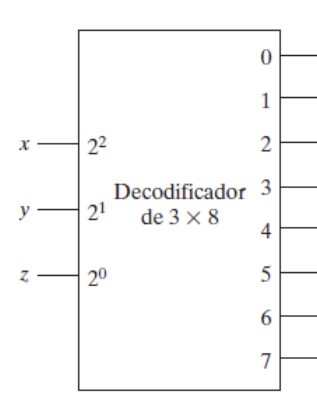
\includegraphics[scale=0.5]{img/3a8.png}
\caption{Decodificador de 3 entradas y 8 salidas}
\end{figure}

La tabla de verdad de un decodificador de 3 entradas y 8 salidas es la siguiente:

\begin{table}[h]
    \centering
    \begin{tabular}{ccc|cccccccc}
        \toprule
        \textbf{X} & \textbf{Y} & \textbf{Z} & \textbf{Y0} & \textbf{Y1} & \textbf{Y2} & \textbf{Y3} & \textbf{Y4} & \textbf{Y5} & \textbf{Y6} & \textbf{Y7}\\
        \midrule
        0 & 0 & 0 & 1 & 0 & 0 & 0 & 0 & 0 & 0 & 0\\
        0 & 0 & 1 & 0 & 1 & 0 & 0 & 0 & 0 & 0 & 0\\
        0 & 1 & 0 & 0 & 0 & 1 & 0 & 0 & 0 & 0 & 0\\
        0 & 1 & 1 & 0 & 0 & 0 & 1 & 0 & 0 & 0 & 0\\
        1 & 0 & 0 & 0 & 0 & 0 & 0 & 1 & 0 & 0 & 0\\
        1 & 0 & 1 & 0 & 0 & 0 & 0 & 0 & 1 & 0 & 0\\
        1 & 1 & 0 & 0 & 0 & 0 & 0 & 0 & 0 & 1 & 0\\
        1 & 1 & 1 & 0 & 0 & 0 & 0 & 0 & 0 & 0 & 1\\
        \bottomrule
    \end{tabular}
\end{table}

\subsubsection{Implementación de lógica con decodificadores}
Un decodificador produce los $2^n$ minitérminos de $n$ variables de entrada. Puesto que cualquier función booleana es susceptible de expresarse como suma de minitérminos, es posible utilizar un decodificador para generar los minitérminos y una compuerta \texttt{OR} externa para formar la suma lógica. Así, cualquier circuito combinacional con $n$ entradas y $m$ salidas se puede implementar con un decodificador de $n$ a $2^n$ líneas y $m$ compuertas \texttt{OR}.

El procedimiento para implementar un circuito combinacional con un decodificador y compuertas OR requiere expresar la función booleana del circuito como suma de minitérminos. Entonces se escoge un decodificador que genere todos los minitérminos de las variables de entrada. Las entradas a cada compuerta \texttt{OR} se escogen de entre las salidas del decodificador, de acuerdo con la lista de minitérminos de cada función.

\newpage
\subsubsection{Ejemplo de Implementación}
Se tiene que implementar la lógica de un sumador completo, la tabla es la siguiente:
\begin{table}[h]
    \centering
    \begin{tabular}{ccc|cc}
        \toprule
        \textbf{A} & \textbf{B} & \textbf{$C_{in}$} & \textbf{S} & \textbf{$C_{out}$}\\
        \midrule
        0 & 0 & 0 & 0 & 0\\
        0 & 0 & 1 & 1 & 0\\
        0 & 1 & 0 & 1 & 0\\
        0 & 1 & 1 & 0 & 1\\
        1 & 0 & 0 & 1 & 0\\
        1 & 0 & 1 & 0 & 1\\
        1 & 1 & 0 & 0 & 1\\
        1 & 1 & 1 & 1 & 1\\
        \bottomrule
    \end{tabular}
\end{table}

De la tabla obtenemos las funciones para el circuito combinacional en forma de suma de minitérminos:

\begin{align*}
    S(x,y,z) &= \sum (1, 2, 4, 7) \\
    C_{out}(x,y,z) &= \sum (3, 5, 6, 7) 
\end{align*}

Puesto que hay tres entradas y un total de ocho minitérminos, se necesita un decodificador de 3 a 8 líneas. El decodificador genera los ocho minitérminos para $x$, $y$, $z$. La compuerta OR de la salida S forma la suma lógica de los minitérminos 1, 2, 4 y 7. La compuerta \texttt{OR} de la salida $C_{out}$ forma la suma lógica de los minitérminos 3, 5, 6 y 7.

\begin{figure}[h]
\centering
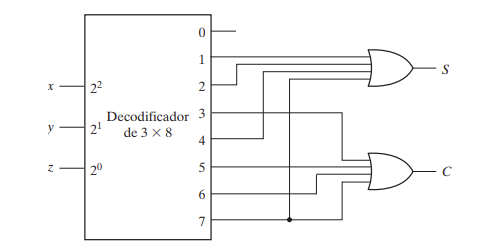
\includegraphics[scale=0.8]{img/sumador.png}
\caption{Implementación de un sumador completo con decodificador}
\end{figure}